\chapter{Results} \label{results}
The results are divided into four sections.
In section \ref{results:detection} the results of the detection algorithm are presented.
In section \ref{results:measuring} the results of the measuring algorithm are presented.
In section \ref{results:overall} the results of detection and measuring combined are presented.
Finally, in section \ref{results:online} the results of online testing are presented

\section{Detection} \label{results:detection}
The output of the detection algorithm was compared against ground truth positions of the reference object and package corners, as explained in \ref{benchmarking}.
The error was defined as the sum of distances between the detected points and actual points, divided by the length of the contour.
A detection result was considered to be correct if the error was less than $10\%$.
Table \ref{table:detection_overall} shows the success rates and average error of the detection algorithm on the set of 225 example image.

\begin{table}%[H]
\centering
\begin{tabular}{@{} l *3c @{}}
\toprule
 & {Reference Object}  & {Package}  & {Reference Object and Package}  \\ 
\midrule
Success rate & 0.72 & 0.66 & 0.60 \\ 
Average error & 0.04 & 0.02 & \\
\bottomrule
 \end{tabular}
 \caption{Success rate and average error of detection.}
\label{table:detection_overall}
\end{table}

Table \ref{table:detection_categories} shows the success rates of detection grouped by four categories: package, rotation, distance, and height. Table \ref{table:detection_categories_error} shows the average error grouped in the same way.

\begin{table}[H]
\centering
\begin{tabular}{lcccc}
\toprule
\multicolumn{2}{c}{Category} & Reference Object & Package & Both\\
\midrule

\multirow{5}{*}{Package} 
& 1 & 0.73 & 0.49 & 0.47 \\ 
& 2 & 0.73 & 0.64 & 0.62 \\
& 3 & 0.78 & 0.93 & 0.76 \\
& 4 & 0.62 & 0.53 & 0.49 \\
& 5 & 0.71 & 0.69 & 0.67 \\
\midrule

\multirow{5}{1.5cm}{Horizontal angle}
& Long side		& 0.56 & 0.53 & 0.38 \\ 
& Angle long		& 0.73 & 0.78 & 0.69 \\
& Wide angle 		& 0.91 & 0.87 & 0.87 \\
& Angle short 	& 0.76 & 0.69 & 0.67 \\
& Short side		& 0.62 & 0.42 & 0.40 \\
\midrule
\multirow{3}{*}{Distance ($m$)} 
& 1 			& 0.56 & 0.53 & 0.38 \\ 
& 1.5  			& 0.73 & 0.78 & 0.69 \\
& 2 			& 0.91 & 0.87 &0.87 \\
\midrule
\multirow{3}{*}{Height} 
& Low 		& 0.51 & 0.44 & 0.37 \\ 
& Medium 	& 0.80 & 0.75 & 0.72 \\
& High		& 0.84 & 0.79 & 0.71 \\
\bottomrule
 \end{tabular}
 \caption{Success rate of detection by grouped by different categories.}
\label{table:detection_categories}
\end{table}


\begin{table}%[H]
\centering
\begin{tabular}{lccc}
\toprule
\multicolumn{2}{l}{Category} & Reference Object & Package\\
\midrule

\multirow{5}{*}{Package} 
& 1 & 0.04 & 0.02\\ 
& 2 & 0.04 & 0.03\\
& 3 & 0.04 & 0.03\\
& 4 & 0.04 & 0.01\\
& 5 & 0.04 & 0.03\\
\midrule

\multirow{5}{*}{Rotation}
& Frontal long		& 0.03 & 0.03 \\ 
& Sharp long	& 0.04 & 0.02 \\
& Wide angle 	& 0.04 & 0.02 \\
& Sharp short 	& 0.04 & 0.02 \\
& Frontal short	& 0.04 & 0.03 \\
\midrule
\multirow{3}{*}{Distance ($m$)} 
& 1 			& 0.03 & 0.02  \\ 
& 1.5  			& 0.04 & 0.02  \\
& 2 			& 0.05 & 0.03  \\
\midrule
\multirow{3}{*}{Height} 
& Low 		& 0.04 & 0.02 \\ 
& Medium 	& 0.04 & 0.02 \\
& High		& 0.04 & 0.02 \\
\bottomrule
 \end{tabular}
 \caption{Average relative error of detection by grouped by different categories.}
\label{table:detection_categories_error}
\end{table}


From table \ref{table:detection_categories} it can be concluded that the success rate of detection varied significantly between the entries in each category.
The frontal views yielded a much lower success rate than the other views.
The same can be said for the furthest distance, and the lowest height. 
From table \ref{table:detection_categories_error} it can be concluded that the relative error did not vary much.
The error was consistently lower for the package than the reference object. % TODO poorly chosen error metric, redo if time

\section{Measuring} \label{results:measuring} 
Measuring results were obtained by using ground truth positions of the corners as input to the measuring algorithm, and comparing the output against the real dimensions of the packages.
The error of each measurement was defined as the sum of relative errors of the three dimensions.
The error was measured as sum of relative errors.
A measurement was considered to be correct if no individual dimension of the package had a relative error greater than $10\%$.

Table \ref{table:measuring_overall} shows the success rate and average error of the two calibration methods.

\begin{table}%[H]
\centering
\begin{tabular}{@{} *3c @{}}
\toprule
&{Vanishing point calibration} & {Zhang's method}\\ 
\midrule
Success rate & 0.81 & 0.93 \\ 
Error & 0.07 & 0.07 \\
\bottomrule 
 \end{tabular}
 \caption{Success rate and average error of measuring.}
\label{table:measuring_overall}
\end{table} % TODO split error into x,y,z

Table \ref{table:measuring_categories} and \ref{table:measuring_categories_error} show the success rate and average error grouped in the same was as in the previous section.

\begin{table}%[H]
\centering
\begin{tabular}{lccc}
\toprule
\multicolumn{2}{l}{Category} & Uncalibrated & Calibrated\\
\midrule

\multirow{5}{*}{Package} 
& 1 & 0.87 & 0.89 \\
& 2 & 0.84 & 0.98 \\
& 3 & 0.84 & 0.96 \\
& 4 & 0.71 & 1.00 \\
& 5 & 0.78 & 0.93 \\
\midrule

\multirow{5}{*}{Rotation}
& Frontal long		& 0.56 &  0.84 \\ 
& Sharp long		& 0.84 &  0.91 \\
& Wide angle 		& 0.98 &  0.98 \\
& Sharp short 		& 0.98 &  1.00 \\
& Frontal hort		& 0.69 &  0.93 \\
\midrule
\multirow{3}{*}{Distance ($m$)} 
& 1 			& 0.89 & 1.00   \\
& 1.5  			& 0.81 & 0.96   \\
& 2 			& 0.72 & 0.84   \\
\midrule
\multirow{3}{*}{Height} 
& Low 		& 0.80 & 0.87  \\
& Medium 	& 0.81 & 0.95  \\
& High		& 0.81 & 0.99  \\
\bottomrule
 \end{tabular}
 \caption{Success rate of measuring by grouped by different categories.}
\label{table:measuring_categories}
\end{table}

\begin{table}%[H]
\centering
\begin{tabular}{lccc}
\toprule
\multicolumn{2}{l}{Category} & Vanishing point calibration & Zhang's method\\
\midrule

\multirow{5}{*}{Package} 
& 1 & 0.09 & 0.08 \\
& 2 & 0.07 & 0.06 \\
& 3 & 0.07 & 0.06 \\
& 4 & 0.07 & 0.07 \\
& 5 & 0.05 & 0.06 \\
\midrule

\multirow{5}{*}{Rotation}
& Frontal long	& 0.08 & 0.08 \\\ 
& Sharp long	& 0.07 & 0.07 \\
& Wide angle 	& 0.07 & 0.07 \\
& Sharp short 	& 0.07 & 0.07 \\
& Frontal short	& 0.07 & 0.07 \\
\midrule
\multirow{3}{*}{Distance ($m$)} 
& 1 			& 0.07 & 0.06 \\
& 1.5  			& 0.07 & 0.07 \\
& 2 			& 0.08 & 0.08 \\
\midrule
\multirow{3}{*}{Height} 
& Low 		& 0.07 & 0.07 \\ 
& Medium 	& 0.07 & 0.07 \\
& High		& 0.07 & 0.07 \\
\bottomrule
 \end{tabular}
 \caption{Average error of measuring by grouped by different categories.}
\label{table:measuring_categories_error}
\end{table}


The results in table \ref{table:measuring_categories} are somewhat similar to the corresponding detection results.
The two frontal views yielded lower success rates, especially for vanishing point calibration.
Success rates also decreased as distance increased.
Table \ref{table:measuring_categories_error} showed that the offline calibration method yielded slightly lower error than vanishing point calibration.

\section{Overall Performance} \label{results:overall}
The results in this section present the performance of the detection and measuring algorithms combined, using vanishing point calibration.
The errors are defined in the same way as in section \ref{results:measuring}.

Table \ref{table:overall_overall} shows the overall performance of detection and measuring combined.

\begin{table}%[H]
\centering
\begin{tabular}{@{} *2c @{}}
\toprule
 & {Overall performance}\\ 
\midrule
Success rate	& 0.51 \\ 
Error 			& 0.07 \\
\bottomrule 
 \end{tabular}
 \caption{Success rate and average error of detection and measuring combined.}
\label{table:overall_overall}
\end{table}

Table \ref{table:overall_categories} and \ref{table:overall_categories_error} show the success rate and average error of detection and measuring combined.

\begin{table}%[H]
\centering
\begin{tabular}{lcc}
\toprule
\multicolumn{2}{l}{Category} & Success rate\\
\midrule

\multirow{5}{*}{Package} 
& 1 & 0.40  \\
& 2 & 0.58  \\
& 3 & 0.62  \\
& 4 & 0.40  \\
& 5 & 0.56  \\
\midrule

\multirow{5}{*}{Rotation}
& Frontal long		& 0.18 \\ 
& Sharp long		& 0.64 \\
& Wide angle 		& 0.82 \\
& Sharp short 		& 0.62 \\
& Frontal hort		& 0.29 \\
\midrule
\multirow{3}{*}{Distance ($m$)} 
& 1 			& 0.57 \\
& 1.5  			& 0.64 \\
& 2 			& 0.32 \\
\midrule
\multirow{3}{*}{Height} 
& Low 		& 0.31 \\
& Medium 	& 0.67 \\
& High		& 0.56 \\
\bottomrule
 \end{tabular}
 \caption{Overall success rate by grouped by different categories.}
\label{table:overall_categories}
\end{table}

\begin{table}%[H]
\centering
\begin{tabular}{lcc}
\toprule
\multicolumn{2}{l}{Category} & Error\\
\midrule

\multirow{5}{*}{Package} 
& 1 & 0.08  \\
& 2 & 0.06  \\
& 3 & 0.06  \\
& 4 & 0.07  \\
& 5 & 0.07  \\
\midrule

\multirow{5}{*}{Rotation}
& Frontal long		& 0.08 \\ 
& Sharp long		& 0.08 \\
& Wide angle 		& 0.05 \\
& Sharp short 		& 0.07 \\
& Frontal hort		& 0.10 \\
\midrule
\multirow{3}{*}{Distance ($m$)} 
& 1 			& 0.07 \\
& 1.5  			& 0.07 \\
& 2 			& 0.08 \\
\midrule
\multirow{3}{*}{Height} 
& Low 		& 0.08 \\
& Medium 	& 0.07 \\
& High		& 0.07 \\
\bottomrule
 \end{tabular}
 \caption{Overall error by grouped by different categories.}
\label{table:overall_categories_error}
\end{table}

The results are similar to those of the individual parts, as expected.
The lower success rates of the frontal views, the furthest distance and the lowest height, are even more prominent in this case.
The results of disregarding these poorly performing positions and only considering the remaining positions are shown in table \ref{table:overall_good}.

\begin{table}%[H]
\centering
\begin{tabular}{@{} *2c @{}}
\toprule
 & {Overall performance}\\ 
\midrule
Success rate	& 0.92 \\ 
Error 			& 0.06 \\
\bottomrule 
 \end{tabular}
 \caption[Improved overall success rate and average error of the system, when some positions are disregarded]{Success rate and average error of detection and measuring combined, while disregarding the poorly performing positions. The disregarded positions are the frontal views, where only two sides of the package can be seen, the furthest distance (2 metres), and the lowest height (0.9 or 1.1 metres). }
\label{table:overall_good}
\end{table}

Table \ref{table:overall_good} shows that disregarding a few of the positions results in a considerably better performance.

\section{Online testing} \label{results:online}

Online testing was performed using the Android application described in \ref{method:online_testing}.
A screenshot of the resulting application is shown in figure \ref{fig:screenshot}. % TODO add more screenshots
The processing time of the application was typically around 300 milliseconds at the resolution $800 \times 450$ on the Galaxy S6 Edge, depending on the amount of clutter in the image. 
More clutter resulted in higher processing times.

% 1000 ms at 1280x720

\begin{figure}[H]
\begin{center}
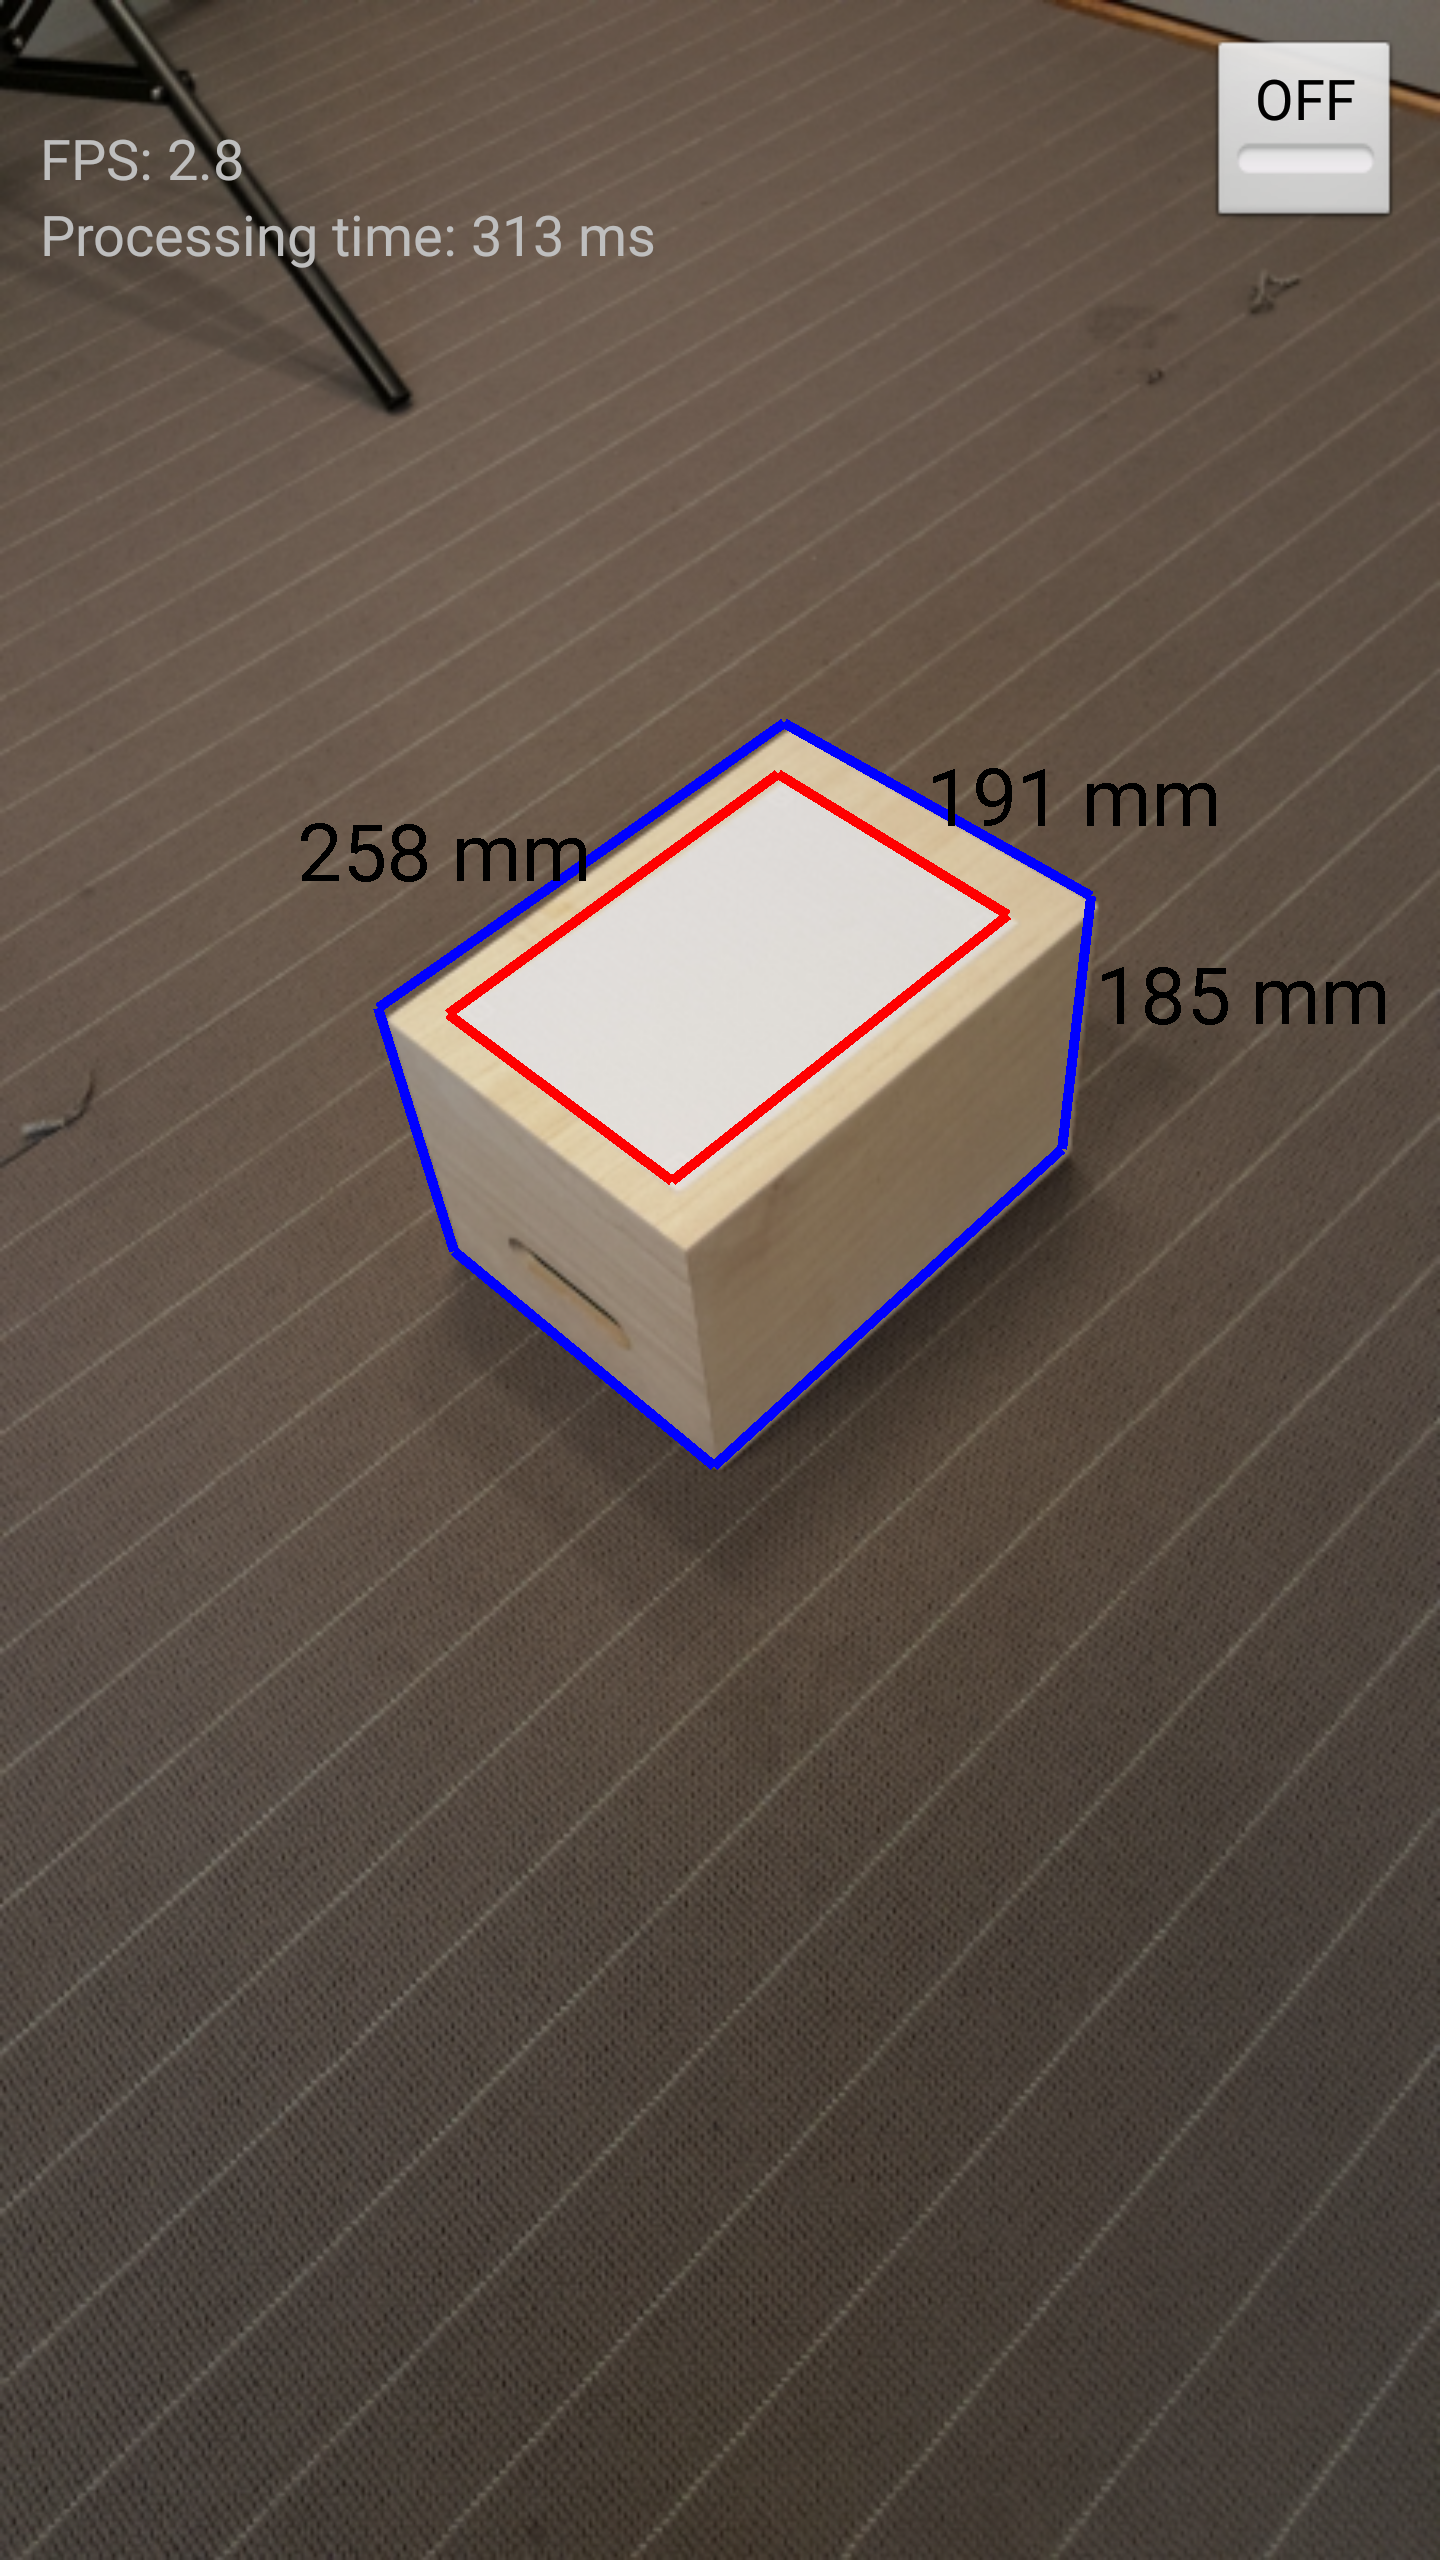
\includegraphics[width=0.6\textwidth]{figures/screenshot.png}
\end{center}
\caption{Screenshot of the app measuring package 2. A blue outline has been drawn around the package, and a red outline has been drawn around the reference object. The real dimensions of the package are $260 \times 191 \times 177$ mm.}
\label{fig:screenshot}
\end{figure}
